\documentclass[12pt,a4paper,notitlepage]{article}

\usepackage{./styles/plog1}

\addbibresource{plog1.bib}

\newcommand*{\foottitle}{Pente}
\newcommand*{\boardsize}[1]{#1\texttt{x}#1}


\title{
	\vspace{-2\baselineskip}
	
\includegraphics[scale=0.15]{feuplogo.jpg}\\
	{\Huge Pente}\\
	{\Large Game Overview, History, Rules and Implementation}\\
	{\normalsize PLOG 2018}
}

\author{
	Bruno Dias da Costa Carvalho\hspace*{1.5em}\text{up201606517}
	\and
	Amadeu Prazeres Pereira\hspace*{1.5em}\text{up201605646} 
}

\begin{document}
\maketitle
\thispagestyle{empty}

\section{Introduction}
\label{sec:introduction}

This project's objective is for us to implement a board game (for us is Pente) using Prolog, with 3 different modes: Player vs Player, Player vs Bot and Bot vs Bot, with the Bot having 2 different difficulties.
  It is needed for us to implement all the game's rules and use the best suiting compounds to represent the game, with the board, pieces, player's turn, etc...
This will all be discussed below.

\section{Overview and History}
\label{sec:overview}

\textbf{Pente} is an \textit{abstract strategy board game}, played usually by two players, in which the aim is to create an unbroken chain of five stones \emph{or} to capture ten of the enemy's stones.

It was created in 1977 by Gary Gabrel at the restaurant \textsl{Hideaway Pizza}, in Stillwater, Oklahoma, USA.\supercite{pente-wikipedia}
Customers waiting for their orders to arrive would play a variation of the game on checkerboard tablecloths.\supercite{pente-wikipedia}

Some variations allow for more than two independent players, and even teams, to play simultaneously. These require relaxing the winning conditions of the game to accommodate for the increased opposition --- namely requiring only a four-in-a-row for three or four players, and allowing mixed captures for teams.\supercite{pente-winning-moves}

\begin{wrapfigure}[12]{l}[2em]{0.33\textwidth}
	\vspace*{-1\baselineskip}
	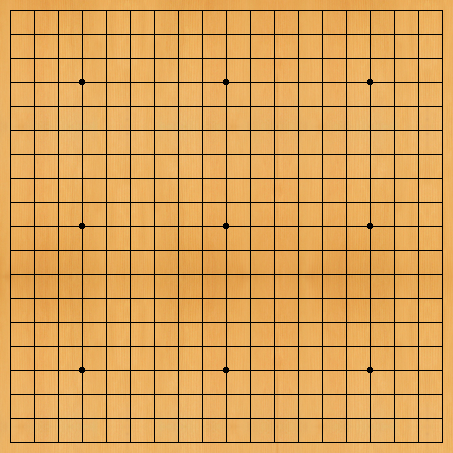
\includegraphics[scale=0.4]{goban.png}
	\caption{\boardsize{19} \textit{Go} board. \label{fig:goban}}
\end{wrapfigure}

The game has many variations for two player games -- all of which have a common ancestry in \textit{Gomoku}, which has a significantly simpler rule-set.
All variations of the game are played in the style of \textit{Go}, on the intersections of a traditional \boardsize{19} \emph{Go} board with black and white pieces called \emph{stones}. One player, \textsl{White}, uses the white stones, and the other, \textsl{Black}, uses the black stones. Once placed on the board, stones may not be moved, but may be removed from the board if \emph{captured}.

Introductory or speed games may be played on the smaller \boardsize{9} or \boardsize{13} boards, but the tighter space makes it very difficult to generate common patterns of play.

\section{Game Rules}
\label{sec:rules}

The game's precise rules vary considerably throughout variations and sources. As such, we'll first review the common base rules and then discuss a few variations.

\subsection{Base rules}
\label{subsec:baserules}

Let's recall there are two winning conditions, same for White and Black:

\begin{itemize}
	\large
	\item Form an unbroken chain of 5 or more consecutive friendly stones --- vertically, horizontally or diagonally.
	\item Capture a total of 10 enemy stones.
\end{itemize}

\begin{wrapfigure}[8]{r}[2em]{0.3\textwidth}
	\vspace*{-3\baselineskip}
	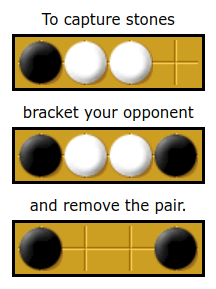
\includegraphics[scale=0.6]{capture.png}
	\caption{Capturing\supercite{pente-net} \label{fig:capture}}
\end{wrapfigure}

Unlike traditional \textit{Gomoku}, the chain may indeed have more than five consecutive stones.

\subsubsection{Captures}
\label{subsubsec:captures}

Captures occur when two friendly adjacent stones (and only two) become bracketed by a pair of enemy stones, in a configuration depicted in \autoref{fig:capture}. Captures may arise in any direction.

\subsection{Variations}
\label{subsec:variations}

Some sources add the following secondary rules.

\begin{itemize}
	\item White always plays first, in the center.\supercite{pente-renjunu, pente-wikipedia} This is unlike \textit{Renju} and \textit{Gomoku}.
	\item \textsl{Suicides} are not possible -- if a player places two adjacent friendly stones into a bracketed position --- for example, if White forms the second panel of \autoref{fig:capture} --- his stones are not captured.\supercite{pente-renjunu,pente-org,pente-wikipedia,pente-winning-moves}
	\item Tournament Rule: The first player's second move is restricted -- it must be at least three intersections away from the center (that is, outside the board's middle \boardsize{5}).\supercite{pente-net,pente-org,pente-wikipedia,pente-winning-moves}
\end{itemize}

We'll be using these three rules hereafter.

Other sources do not specify starting player (or choose Black) and do not require the tournament rule, at least for casual play. 

Among variations we find: suicides allowed, called \textit{poofs} (\textit{Poof-Pente}); harsher Tournament Rule (\textit{G-Pente}, \textit{D-Pente}); 3-in-a-row captures (\textit{Keryo-Pente}), and others.\supercite{pente-org,pente-net}

\section{Implementation: Internal Representation}
\label{sec:internal}

Representing the game's board is fairly simple. Every position in the SxS board is in one of three states: white piece, black piece, or empty. We'll represent the board using a SxS matrix (list of lists), whose elements are \textbf{w}, \textbf{b} or \textbf{c}, for each state respectively. This matrix will be called $Board$.

Now, each player has captured a certain number of pieces (an integer) and only plays pieces of a certain color (white or black). We'll represent the captures as a pair $[Wc,Bc]$, with no similar abstraction for players.

The overall game state will be kept by $\textup{game}(Board, P, [Wc,Bc], Turn, Options)$, where P is \textbf{w} or \textbf{b} according to who will play next, Turn is an integer representing the current game turn number, starting at 0. Lastly, Options is a list with the game options (this will be discussed next).

\section{Implementation: Board Display}
\label{sec:boarddisplay}

It's possible to flip the board (display only, not representation) when it is Black's turn to play, as if the two players were playing face-to-face on a physical Go board. Naturally we adjust the identification of rows and columns.

To draw the board with text (on the console) we used unicode box-drawing characters (range \texttt{u+2500}--\texttt{u+257f}). The white and black pieces become filled and empty unicode circles, respectively.

\begin{figure}[bhtp]
	\begin{minipage}{0.45\textwidth}
	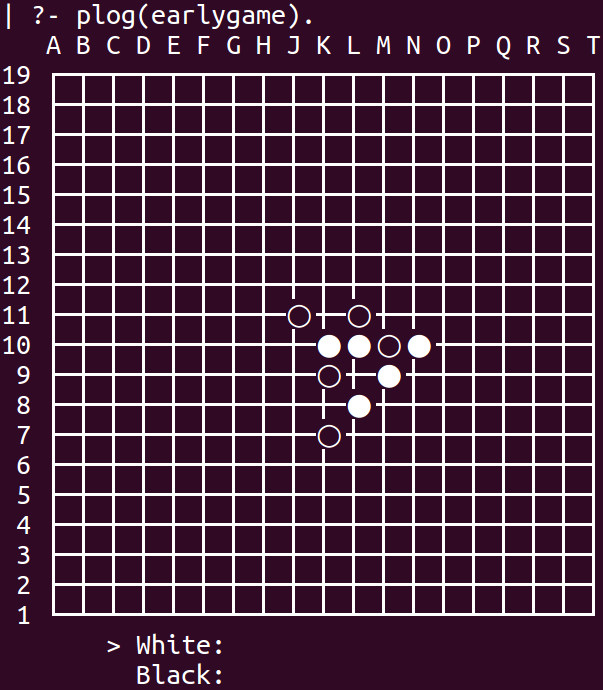
\includegraphics[scale=0.25]{earlygame.png}
	\end{minipage}
	\begin{minipage}{0.55\textwidth}
		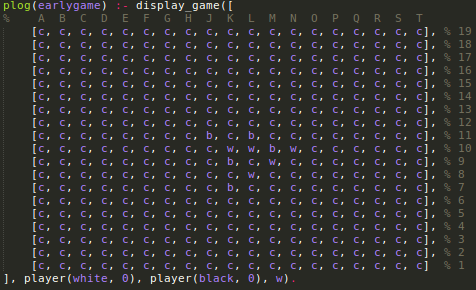
\includegraphics[scale=0.50]{earlygame-code.png}
	\end{minipage}
	\caption{A game after 10 moves. It is White's turn to play.\label{fig:earlygame}}
\end{figure}

\begin{figure}[bhtp]
	\begin{minipage}{0.45\textwidth}
		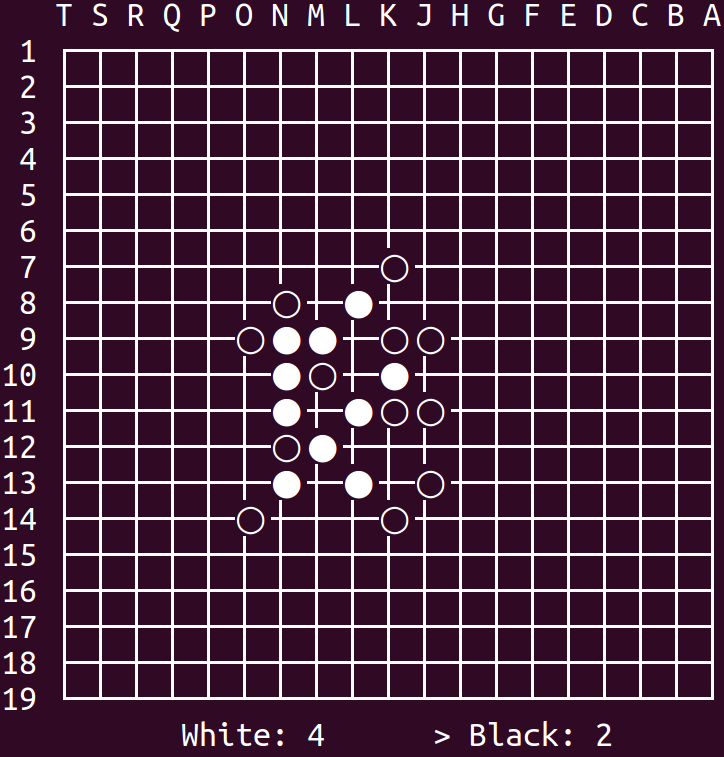
\includegraphics[scale=0.25]{midgame.png}
	\end{minipage}
	\begin{minipage}{0.55\textwidth}
		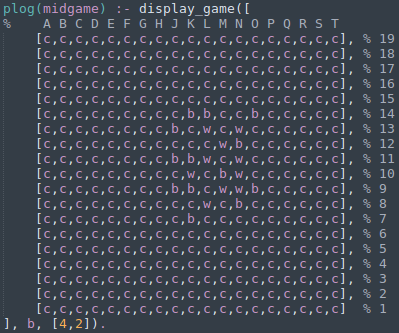
\includegraphics[scale=0.50]{midgame-code.png}
	\end{minipage}
	\caption{A game after 29 moves. It is Black's turn to play.\label{fig:midgame}}
\end{figure}

\begin{figure}[bhtp]
	\begin{minipage}{0.45\textwidth}
		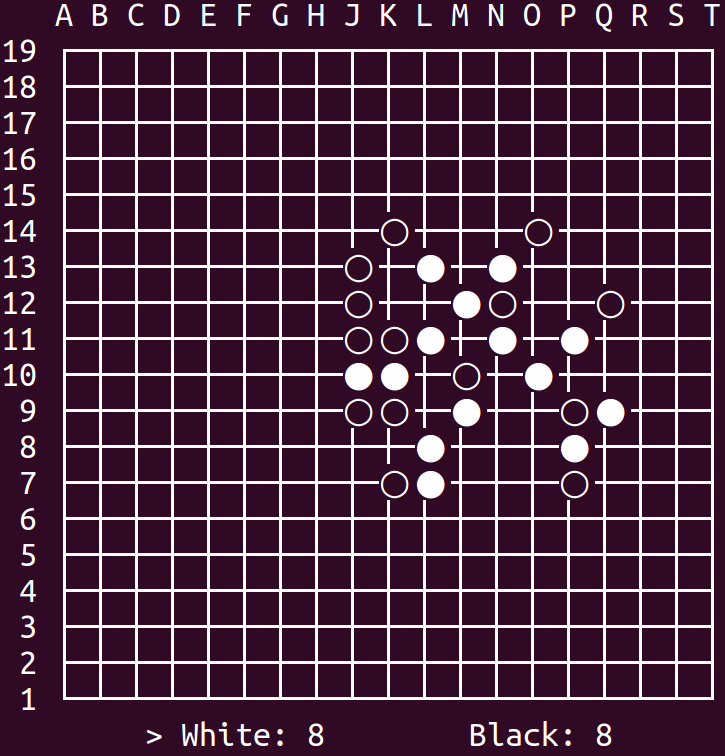
\includegraphics[scale=0.25]{lategame.png}
	\end{minipage}
	\begin{minipage}{0.55\textwidth}
		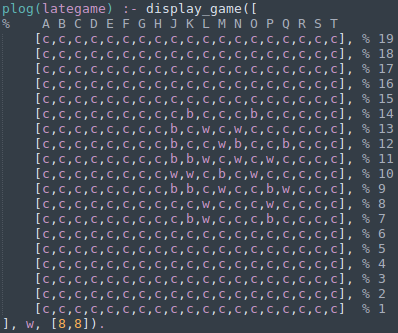
\includegraphics[scale=0.50]{lategame-code.png}
	\end{minipage}
	\caption{A game after 44 moves. It is White's turn to play, and win at H11.\label{fig:lategame}}
\end{figure}

\section{Options}

The overall game state will be represented by a $game/5$ compound. This compound is game(Board, P, [Wc, Bc], Turn, Options), where P is w or b according to who will play next, Turn is an integer thst represents the current game turn number, starting at 0. Lastly, Options is a list that represents the game's options. These option include (use 'help' to get same information): 

\begin{itemize}
	\item \textbf{board\_size(S)} or size(S), S in {7,9,11,...}\\
	Defines the board size (SxS), must be odd.
	Default: 19
	\item \textbf{difficulty(D)}, D in {1,2,3,4,5}\\
	Sets the bot difficulty (with 5 being the most
	difficult) by selecting a set of predefined values
	for depth, padding and width. If given values for
	depth, padding and width, these override those selected
	by the difficulty.
	Default: 3
	\item \textbf{depth(D)}, D in {0,1,2,3,...}\\
	Depth of the bot search tree.
	Suggestion: Choose an even depth (2 or 4).
	Default (difficulty 3): 5
	\item \textbf{padding(P)}, P in {0,1,2,3,...}\\
	Padding of the active subboard used by the search tree.
	Default (difficulty 3): 2
	\item \textbf{width([W0,W1,...])}, Wi in {1,2,3,...}\\
	For each search node on depth i (top is depth 0)
	recurse the search tree only for the Wi best moves.
	If the width is not defined for all the depths, the
	last width in the list will be used repeatedly.
	- width(W), W in {1,2,3,...}
	Use the width W for all depths.
	Default (difficulty 3): [4,3,2]
	\item \textbf{flip\_board(B)} or \textbf{flip(B)}, \textbf{B} is true or false\\
	Flip the board print on the console for Blacks turn.
	Default: false
	\item \textbf{tournament\_rule(B)} or \textbf{rule(B)}, \textbf{B} is true or false\\
	Use the tournament rule.
	Default: true
\end{itemize}

\subsection{Valid Moves}
\label{subsec:validmoves}

In Pente, the player's possible moves does not depend on which player is going to play. The available moves are the same for each one.
With this being said we implemented several predicates that give us a list with all the possible moves a player can make.

\begin{itemize}
	\item \textbf{valid\_moves/2}\\
	This gives the player all the empty positions on the board, does not take in consideration the game's turn or if the user wants to play using the tournament rule.
	\item \textbf{valid\_moves/3}\\
	Being more specific than the previous one it takes a given turn making sure that at the turn number 0 the only available move for the player is the center piece.
	By default it uses the Tournament rule at turn 2.
	\item \textbf{valid\_moves/4}\\
	Takes into account the game turn and if the tournament rule is active or not. At turn 0 the only valid move is still the center one, and at turn 2 if the Tournament rule is being used the valid moves are the empty positions at least 3 intersections away from the center.
\end{itemize}

\subsection{Validation and Execution of Moves}
\label{subsec:moves}

When a player makes a move it needs to be checked. This analysis is made seeing if the player move is in the appropriate list of valid moves, as returned from one of the predicates described above.

In the case that the player move is valid we do several things:

\begin{enumerate}[label=(\alph*)]
	\item Place the player's corresponding colored stone at the given game coords.
	\item Check if that stone bracketed the opponent, in each of the possible eight directions. Then add 2 captures to the player's captures and remove those 2 stones from the board.
	\item Update the next player playing.
	\item Increment the game's turn by 1.
\end{enumerate}

This is all done in \textbf{move/3}.

\subsection{Game Over}
\label{subsec:gameover}

In the end of every game iteration a test is performed by \textbf{game\_over/2} to check for either winning condition, for either player.

In case of victory, a message is displayed for that player and the game cycle is stopped, finishing the game successfully. Otherwise the game goes on naturally.

\subsection{Board Scoring}
\label{subsec:boardscoring}

The board evaluation is based on list patterns. No two-dimensional patterns are recognized or searched for when evaluating a board; rather, patterns are searched in lists --- all the board's rows, columns, and diagonals. Each reasonable sized pattern comprised solely of one player's pieces is scored by \textbf{pattern/2} and \textbf{score/2} to be of an integer value between $1$ and $2^{100}$, the former for a single stone and the latter for a five-in-a-row. Every pattern is then counted in every list, scoring said list as a weighed sum of the number of patterns it contains.

Patterns made with White pieces are positive, those made with Black pieces are symmetrical. After scoring each list with \textbf{evaluate/2}, the Board's total value is the sum of the list scores (\textbf{evaluate\_board/2}). The value of a game position is the Board's value, plus a bonus for the number of captures of either player.

There are about $150$ patterns scored by hand, for a total of $300$ pattern searches in every list. Some of these are not very meaningful and can be removed to increase efficiency, but we did other things to speed up evaluation:

\begin{itemize}
	\item Instead of evaluation an entire board every time with \textbf{evaluate\_board/2}, we use mostly \textbf{reevaluate\_board} which takes two Boards that differ by just one stone placement, the initial Board's value, and computes the new Value, only having to reevaluate, most of the time, four new lists.
	\item Predicate \textbf{evaluate/2} is dynamic and every list evaluation
	is stored using \textbf{asserta} (the lemma idiom). This results in thousands of clauses, and evaluation is mostly replaced by lookup, but the speed is very considerable.
\end{itemize}

\subsection{Computer Bot Moves}
\label{subsec:bot}

We made an elaborate, although largely imperfect and static bot to play the game which uses a mix of a lookahead analysis tree and board evaluations.

The analysis tree simulates moves on the board to evaluate and inspect possible future positions. This is done recursively to a variable depth (the lookahead length) and mostly depth-first, and variable width (number of children per node). Future positions which are winning or losing positions are identified and handled specially; other positions are merely scored by board evaluation and ranked. From the best moves, one at random is chosen and played.

From our experience, difficulty 3 gives a bot which computes reasonably fasts, makes decent moves, and answers most forcing moves adequately.

For reference, see predicates \textbf{build\_children/3} and \textbf{recurse\_children/3}.

\subsection{Conclusion}

This project required a lot of work, but was very rewarding.
We achieved everything that we stipulated from the beginning and plenty more. In our opinion we took what was asked for and elevated it to another level giving the player a lot more options to customize both bot and the game.
The biggest difficulties when developing this game was, definitely, the making of the Bot's evaluation tree. It has some faults (obviously it doesn't resign, for instance), but we think we conquered this and are pretty happy with how it turned out.
The one thing that we would like to improve are the values for each pattern, in our opinion these aren't perfectly tuned and would require more time to perfect these.

\printbibliography

\end{document}